\chapter{Method of work}
\label{chap:method}
\drop{I}{n} this chapter, the development software methodology applied for carrying
out this project is described. Furthermore, the tools such as hardware and software used are enumerated.
 
\section{Development Methodology}
The selected methodology is based in the \emph{Iterative and Incremental}
model. This model provides numerous advantages such as early adaptability,
continuously testing and has an implementation implementation close to the final product. A
scheme of the model is shown in figure~\ref{fig:IncrementalModel}.


\begin{figure}[!h]
\begin{center}
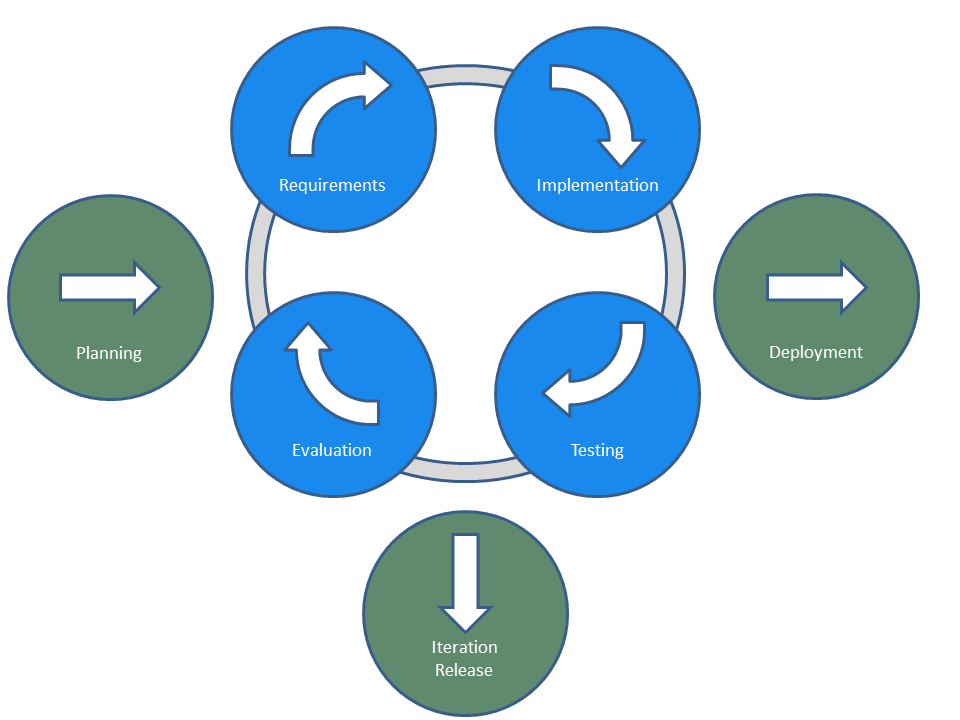
\includegraphics[width=0.8\textwidth]{statement/IterativeIncrementalDevelopment.png}
%http://www.meranetworks.com/services/processes/iterative
\caption{Iterative-Incremental model scheme}
\label{fig:IncrementalModel}
\end{center}
\end{figure}

This methodology enforces a strategy based in small iterations. In each
iteration, the analisys of the requirements, implementation, testing and
evaluation of the product is done. This permits to generate a prototype,
iteratively to approach the final version validating the initial
requirements. Thus, if the advisor requires any changes, they can be easily done.
 
As the project has several parts, it is divided in modules and each module, in iterations. These iterations are explained in Section~\ref{section:evolution}.

\section{Tools used in the project}

In this section the tools and resources used to develop the project are described.  



\subsection{Programming Languages}

Several programming languages were used for the Geo-Cloud
implementation. These languages were described in
Section~\ref{sec:high-level-languages}. They can be
summarized as follows:

\begin{itemize}
\item \textbf{Python:}  it is the main language used in the project. It is a
  multiplatform, multipurpose object oriented language, although it permits imperative and functional
programming. It does not require to compile the source because it is
interpreted.
 \item \textbf{\ac{XML}:} is a mark-up language that defines a set of rules for encoding
documents in a format. It is used in some configuration files thath both the
\emph{Orchestrator} and the User Interface tool use.

\item \textbf{\ac{JSON}:} it is a lightweight language to interchange data between
  applications. The \bonfire experiment descriptor is written in this
  language, indicating the virtual machines instances, physical machines and the
  network resources instantiated.

\item \textbf{Bash:} it consists of several sentences that the operative system can read and translate to play a specific action. All current
\emph{Linux} distributions contain a \emph{Bash} interpreter. 

\end{itemize}


\subsection{Hardware}

The development of the GEO-Cloud project was carried out in a PC provided by
\emph{Elecnor Deimos} with the following features:
\begin{itemize}
\item \emph{Intel Core i5 3450 3.1 GHz}
\item \emph{8 GB RAM}
\end{itemize}

For the Version Control, Bitbucket~\footnote{Official Webpage:
  http:www.bitbucket.org} server and the \emph{Git} version control system were used.

The used resources provided  by the \emph{Fed4FIRE} testbeds are the following:

\begin{itemize}
\item \textbf{PlanetLab}: It currently provides 1204 nodes at 593 sites around
  the world. The selected nodes for carrying out this project are shown in
  Table~\ref{tab:ple-tablelayer1-nodes} and Table~\ref{tab:ple-tablelayer2-nodes}.

\item \textbf{Virtual Wall}: It consists of 100 nodes (dual processor o dual
  core servers) interconnected via a non-blocking 1.5 Tb/s Ethernet switch. 29
  nodes have been used to simulate the satellite constellation and ground
  stations. 

\item \textbf{BonFIRE}: Nodes from diferent testbeds were selected. The
  features the several types of nodes are summarized in Table~\ref{table:intro-instance-types}.
  \begin{itemize}
    \item From INRIA: 2 nodes Medium.
    \item From EPCC: 1 node Xlarge for Orchestrator and a \ac{EaaS} for
      Processing Chain with at least 1  and maximum 60 active Xlarge resources. <<MODIFICABLE>>
    \item From IBBT: 1 Shared Storage.

    \end{itemize}
\end{itemize}


\subsection{Software}

The software  used in the development of this project can be grouped in:
Operative Systems where the software was developed and tested; Software
development tools with which the source was performed;  graphics and documentation
software in which the documentation was carried out; and software libraries
which provide specific functionalities.

\begin{itemize}
\item \textbf{Operative Systems}
\begin{itemize}
\item{\emph{Ubuntu}}: UNIX based operative system in which the development was done. It
  is based in Debian and distributed under \ac{GPL} v3.
\item{\emph{Debian}}: UNIX based operative system distributed under \ac{GPL}
  v3. It provides more than 37500 precompiled software packets which can be
  easily installed. The \bonfire, \vw and \pl virtual machines have this operative system.
\end{itemize}


\item \textbf{Software Development Tools}

\begin{itemize}
\item{\emph{Emacs}}: versatile and powerful text editor developed by Richard
  Stallman. This tool is used with \emph{Pymacs} together. Version used 23.2.
\item{\emph{JFed}}: tool developed by \emph{iMinds}\footnote{Official Webpage: http:www.jfed.iminds.be}(Ghent) for deploying nodes in
  \emph{Fed4FIRE} testbeds. 
\item{\emph{BonFIRE Web Interface}}: \bonfire tool that provides the experiment
  deployment. It can be done manually or automatically using a experiment descriptor.
\item \emph{Ipython}:  command shell for interactive computing in Python. It
  allows us to check some code statements before adding them in a software.
\item \emph{GeoServer}: is an open source software server licensed under the
  \ac{GNU} General Public License, written in \emph{Java} that allows us to
  share and edit geospatial data. Designed for interoperability, it publishes
  data from any major spatial data source using open standards.
\item \emph{Apache Tomcat}:  is an open source software implementation of the \emph{Java Servlet} and \emph{JavaServer Pages} technologies from \emph{Sun Microsystems}, and provides an \ac{HTTP} web server environment for \emph{Java} code to run in, being one of the most popular \emph{Java} application servers~\cite{Foundation2014b}.
\end{itemize}


\item \textbf{Graphics and documentation}

\begin{itemize}
%http://www.latex-project.org/
\item{\emph{\LaTeX}}:is a document mark-up language widely used for the
  communication and publication of scientific documents~\cite{Oetiker2014}. It is multiplatform and is distributed under \ac{GPL} v3.
%http://www.gimp.org/
\item{\emph{GIMP}}: is the \emph{GNU Image Manipulation Program}. It provides photo retouching, image composition and image authoring among
  others. It is multiplatform and is distributed under \ac{GPL} v3.
%http://dia-installer.de/index.html.es
\item{\emph{Dia}}: multiplatform software for drawing many types of
  schemes. Some design schemes of this document were performed on it.
% https://en.libreoffice.org/
\item \emph{Libre Office:} free open source office suite, developed by \emph{The
      Document Foundation}. This suite provides such software as \emph{Draw} and
    \emph{Writer} among other programs. 
\end{itemize}

\item \textbf{Software Libraries}

\begin{itemize}
\item{\emph{Python-mysql}}: \emph{Python} library that provides a high-level interface
  \emph{MySQL} programming. 
\item{\emph{Python-mathplotlib}}: \emph{Python} library that provides some tools and
  functions for plotting and representing data. 
\item{\emph{Python-xml}}:\emph{Python} library used to manage \ac{XML} files.
\item{\emph{Paramiko}}: \emph{Python} library that provides high-level interfaces for
  connecting through \ac{SSH} to other network host. 
\item \emph{PyQt:} Python binding for the \emph{Qt} cross-platform framework. \emph{PyQt} is
  available in two versions, \emph{PyQt4} and \emph{PyQt5}. \emph{PyQt5} was
  used for developing the \acs{GUI} of the project. 
\item \emph{Phonon:} multimedia \ac{API} provided by Qt for handling multimedia
  streams. It was used in the development of the \ac{GUI} for experimentation.
\end{itemize}
\end{itemize}
